\documentclass[tikz,border=15pt]{standalone}
\usepackage{circuitikz}
\usepackage{amsmath}
\begin{document}
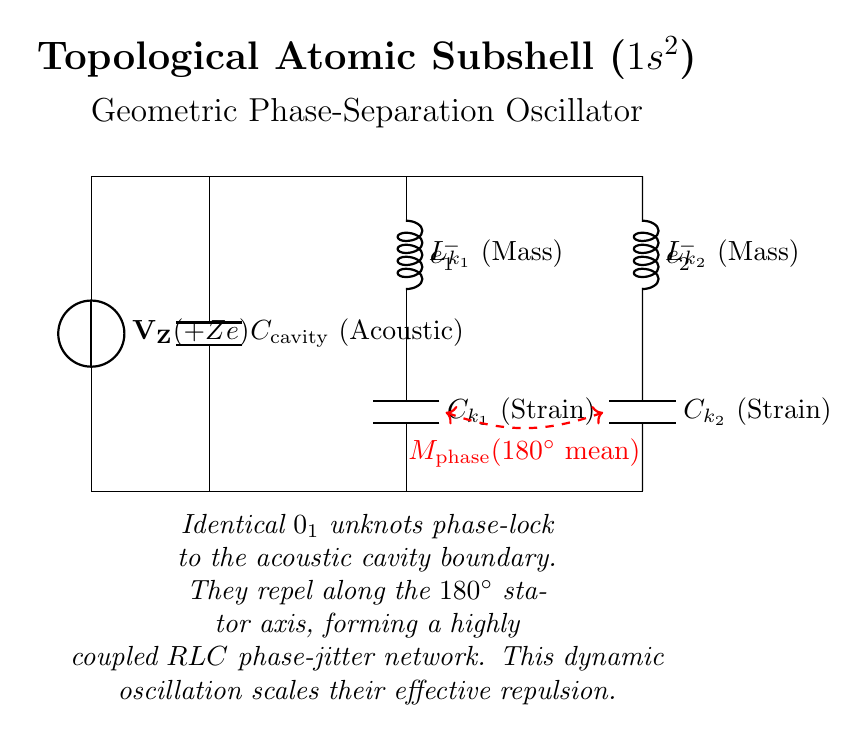
\begin{tikzpicture}
    % Circuit for 1s^2 (Helium) Phase-Jitter LC Oscillator
    
    % Nucleus Stator Core
    \draw (0, 0) to[V, l=$\mathbf{V_{Z}} (+Ze)$] (0, -4);
    \draw (0, 0) -- (1.5, 0);
    \draw (0, -4) -- (1.5, -4);
    \draw (1.5, 0) to[C, l=$C_{\text{cavity}} \text{ (Acoustic)}$] (1.5, -4);
    
    % Electron 1 (Unknot Node A)
    \draw (1.5, 0) -- (4, 0);
    \draw (1.5, -4) -- (4, -4);
    \draw (4, 0) to[L, l=$L_{k_1} \text{ (Mass)}$] (4, -2) to[C, l=$C_{k_1} \text{ (Strain)}$] (4, -4);
    \node at (4.5, -1) {$e^-_1$};
    
    % Electron 2 (Unknot Node B)
    \draw (4, 0) -- (7, 0);
    \draw (4, -4) -- (7, -4);
    \draw (7, 0) to[L, l=$L_{k_2} \text{ (Mass)}$] (7, -2) to[C, l=$C_{k_2} \text{ (Strain)}$] (7, -4);
    \node at (7.5, -1) {$e^-_2$};
    
    % The Phase Interaction (Mutual Inductance Jitter)
    \draw[<->, dashed, red, thick] (4.5, -3) to[bend right=20] node[midway, below] {$M_{\text{phase}} (180^\circ \text{ mean})$} (6.5, -3);
    
    % Diagram Labels
    \node at (3.5, 1.5) {\Large \textbf{Topological Atomic Subshell ($1s^2$)}};
    \node at (3.5, 0.8) {\large Geometric Phase-Separation Oscillator};
    \node[align=center, text width=8cm] at (3.5, -5.5) {
        \textit{Identical $0_1$ unknots phase-lock to the acoustic cavity boundary.\\
        They repel along the $180^\circ$ stator axis, forming a highly\\
        coupled $RLC$ phase-jitter network. This dynamic \\
        oscillation scales their effective repulsion.}
    };
\end{tikzpicture}
\end{document}
